\documentclass{article}

\usepackage{charter} % Use the Charter font
\usepackage[
    a4paper,
    top=1in,
    bottom=1in,
    left=1in,
    right=1in,
]{geometry}

\setlength{\parindent}{0pt}     % Paragraph indentation
\setlength{\parskip}{1em}       % Vertical space between paragraphs

\usepackage[spanish]{babel}
\usepackage{graphicx}
\usepackage{wallpaper}
\usepackage{fancyhdr}
\usepackage{hyperref}
\usepackage{setspace}
\doublespacing

\fancypagestyle{firstpage}{%
    \fancyhf{} % Clear default headers/footers
    \renewcommand{\headrulewidth}{0pt} % No header rule
    \renewcommand{\footrulewidth}{1pt} % Footer rule thickness
}
\fancypagestyle{subsequentpages}{%
    \fancyhf{} % Clear default headers/footers
    \renewcommand{\headrulewidth}{1pt} % Header rule thickness
    \renewcommand{\footrulewidth}{1pt} % Footer rule thickness
}
\AtBeginDocument{\thispagestyle{firstpage}}
\pagestyle{subsequentpages}

\begin{document}
\noindent
\begin{minipage}[t]{0.2\textwidth}
    \vspace*{-2cm}
    \begin{singlespace}
    
\includegraphics[scale=0.06]{images/Logo_UNAM.png}
    \end{singlespace}
\end{minipage}
\hfill
\begin{minipage}[t]{0.8\textwidth}
    \raggedleft
    \begin{tabular}{l @{} }
        Fecha:  6 de abril de 2026\\
        Alumna: Laura Itzel Rodríguez Dimayuga\\
        Cuenta: 422013628\\
        Asesor: M. en Fil. C. Enrique Francisco Soto Astorga
  \end{tabular}
\end{minipage}
% \begin{minipage}[t]{0.2\textwidth}
%     \vspace*{-2.5cm}
%     \begin{singlespace}
%     
\includegraphics[scale=0.06]{images/Logo_FC.png}
%     \end{singlespace}
% \end{minipage}

\vspace{-1em}

\rule{\linewidth}{1pt}

\bigskip

\noindent
A la Comisión de Servicio Social de la Licenciatura en Ciencias de la Computación,\\
Facultad de Ciencias,\\
Universidad Nacional Autónoma de México

\bigskip

Por medio del presente, yo, Laura Itzel Rodríguez Dimayuga, con número de cuenta
422013628, alumna de la Licenciatura en Ciencias de la Computación en la Facultad de Ciencias,
informo las actividades desarrolladas durante mi servicio social, realizado bajo la asesoría del
M. en Fil. C. Enrique Francisco Soto Astorga, en el programa de Apoyo a Difusión y Divulgación
Científica, con clave SSS-2025-12/139-441, registrado ante la DGOAE, en el marco de la
1ra Conferencia Internacional de Filosofía de la Computación 2025.

Desde el 3 de octubre me encargué de promocionar las conferencias a través de redes sociales, 
principalmente Facebook, creando contenido visual y textual para informar sobre los eventos, 
sus fechas, horarios y temas a tratar. Además, ayudé a mantener la página web dedicada a las 
conferencias, donde se publicaron detalles sobre los ponentes, el programa y los materiales 
relacionados. También colaboré en la organización logística de las conferencias, coordinando 
con los ponentes y asegurando que todo el material necesario estuviera disponible para su 
presentación. Para ello, ayudé a revisar las presentaciones, semblanzas y biografías de los 
ponentes, con el fin de catalogar los diferentes bloques que constituyeron los distintos ejes 
temáticos de la conferencia.

Durante el periodo del 27 de octubre al 1 de noviembre, ayudé a registrar a los asistentes, 
además de ser encargada de diversas salas donde presenté a los ponentes, asegurando que las 
conferencias se desarrollaran sin contratiempos técnicos o logísticos. También, durante el 
periodo del 2 al 6 de noviembre, me encargué de recopilar y organizar el material de las 
conferencias para su posterior difusión, incluyendo la edición de fotos y videos para su 
publicación en redes sociales y la página web. Posteriormente, en enero, me encargué de 
recopilar la información sobre los asistentes y la participación de los ponentes para enviar 
sus certificados de participación. Finalmente, durante febrero y marzo, colaboré en la 
redacción de un ensayo divulgativo que servirá como base para videos cortos sobre los temas 
abordados en el Seminario de Filosofía de la Computación, los cuales se publicarán en redes 
sociales con el objetivo de acercar estos contenidos a un público más amplio.
\bigskip
\section*{Evidencia de actividades}
A continuación se presentan capturas de pantalla de las publicaciones realizadas en redes sociales, así como algunos materiales relacionados con la organización y difusión de las conferencias. Estas evidencias demuestran mi participación activa en la promoción, organización y difusión de los eventos, cumpliendo con los objetivos establecidos para el servicio social.
\begin{center}
    \begin{minipage}{0.24\textwidth}
        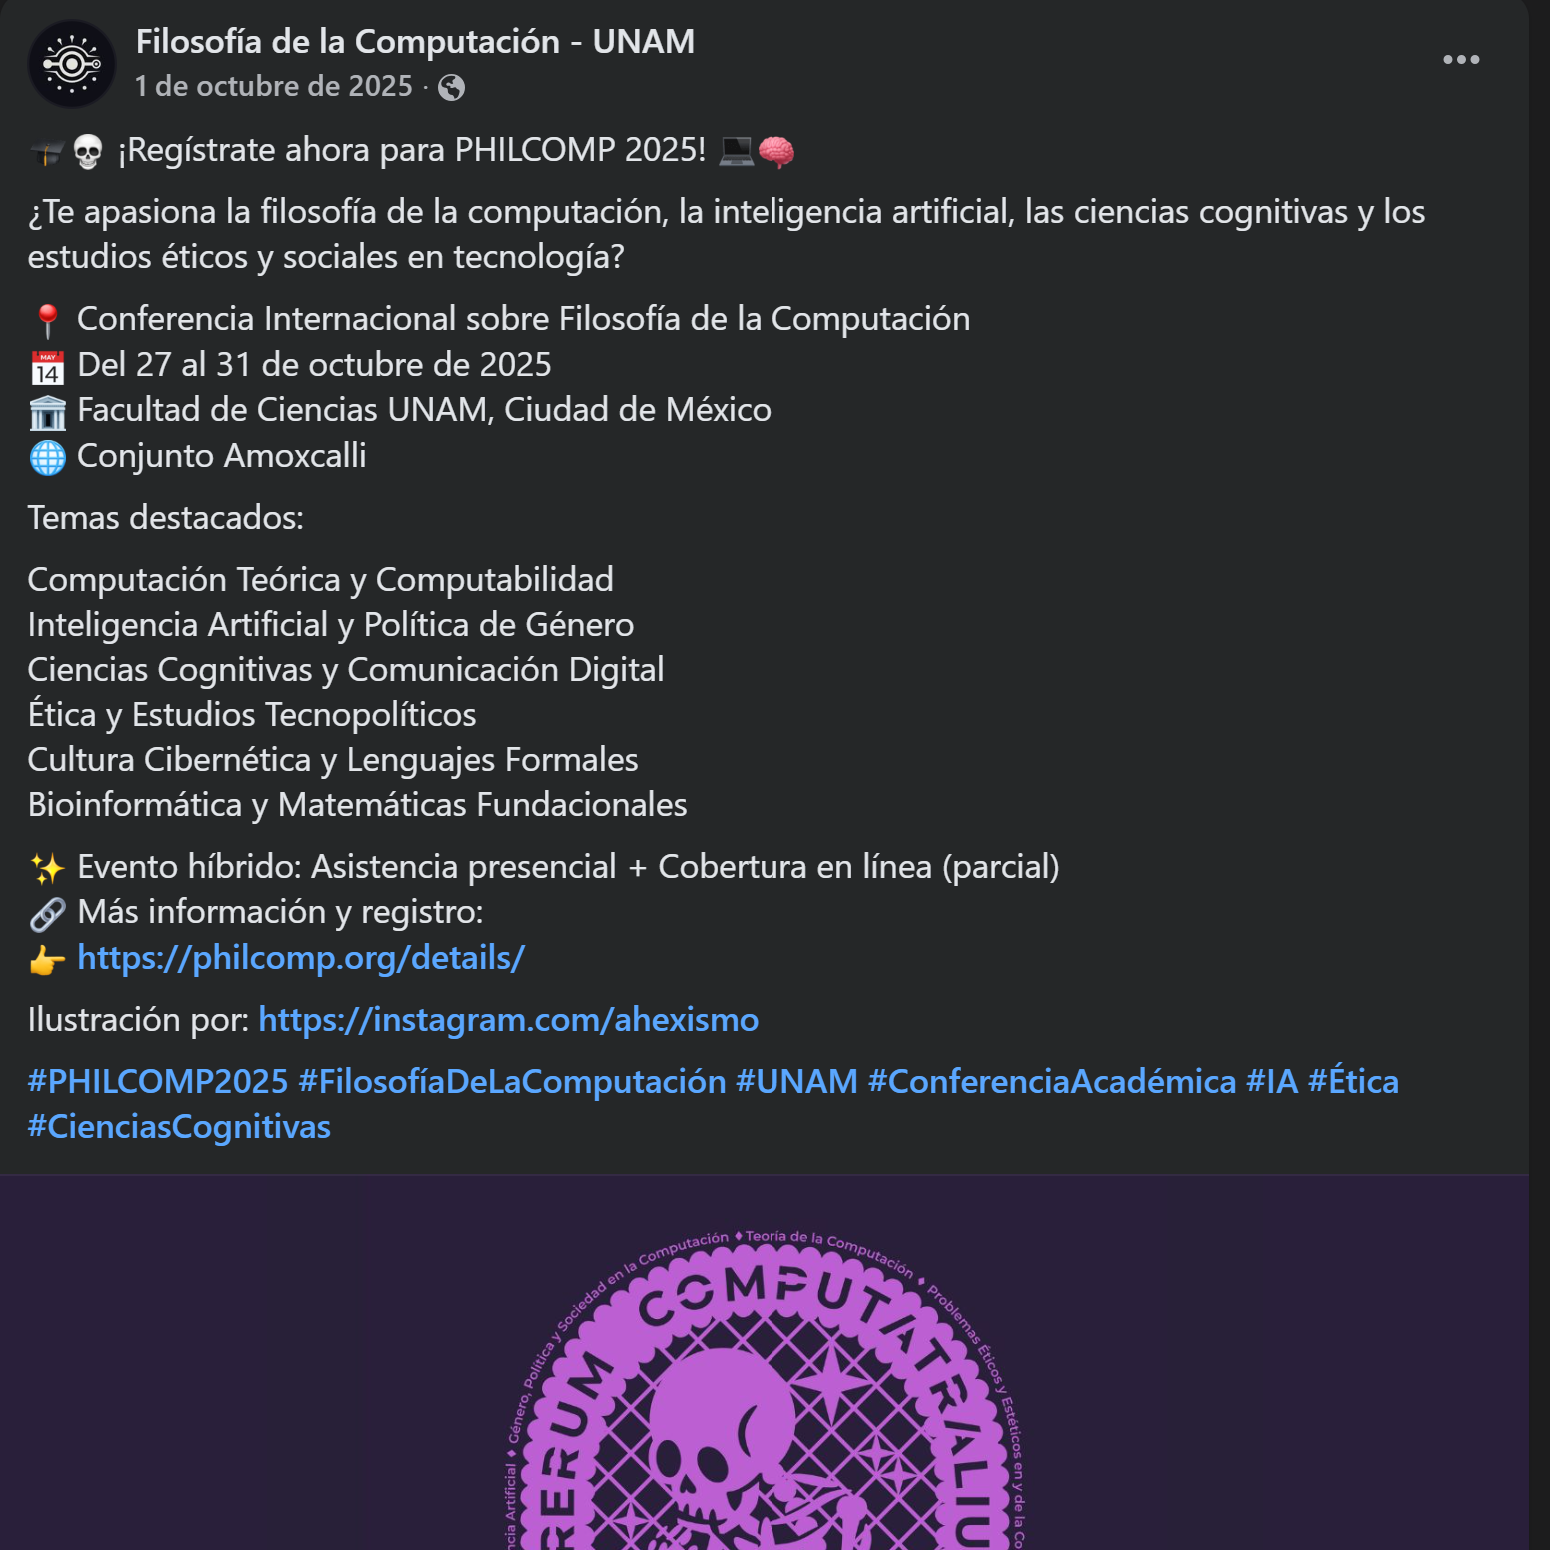
\includegraphics[width=\linewidth]{images/post1.png}
    \end{minipage}\hfill
    \begin{minipage}{0.24\textwidth}
        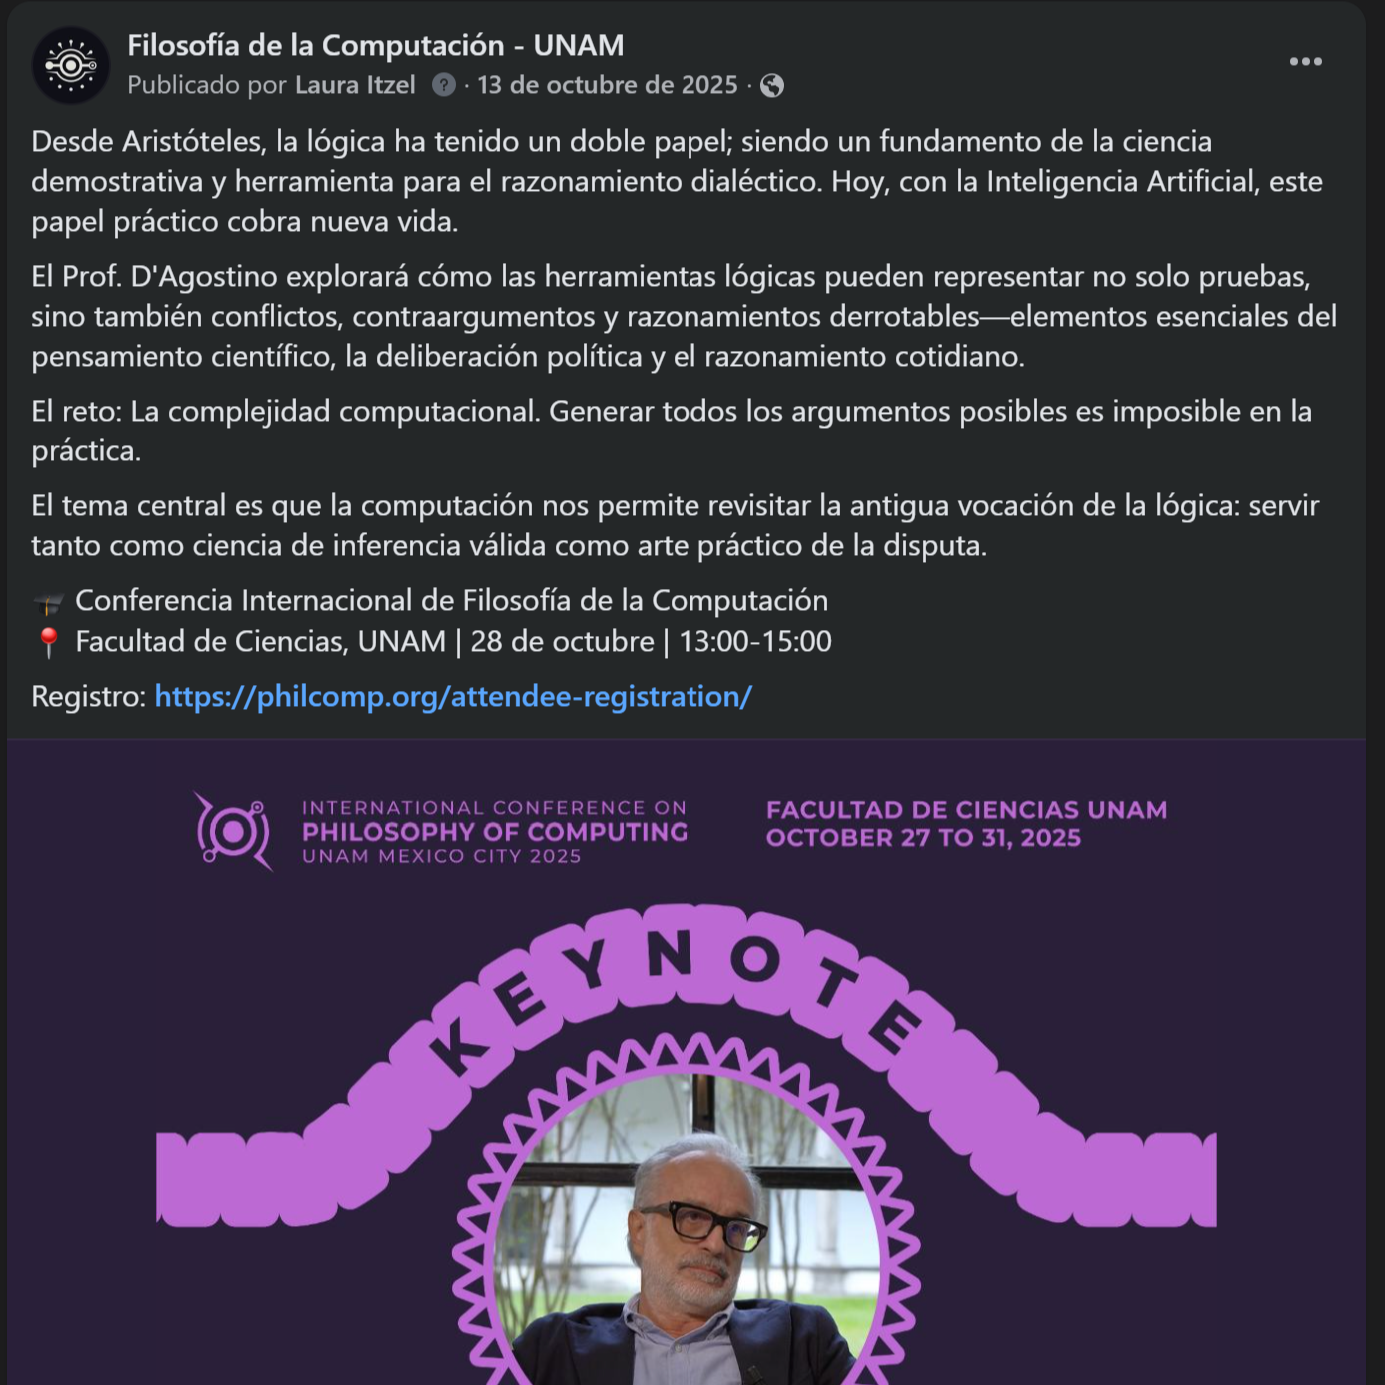
\includegraphics[width=\linewidth]{images/post2.png}
    \end{minipage}\hfill
    \begin{minipage}{0.24\textwidth}
        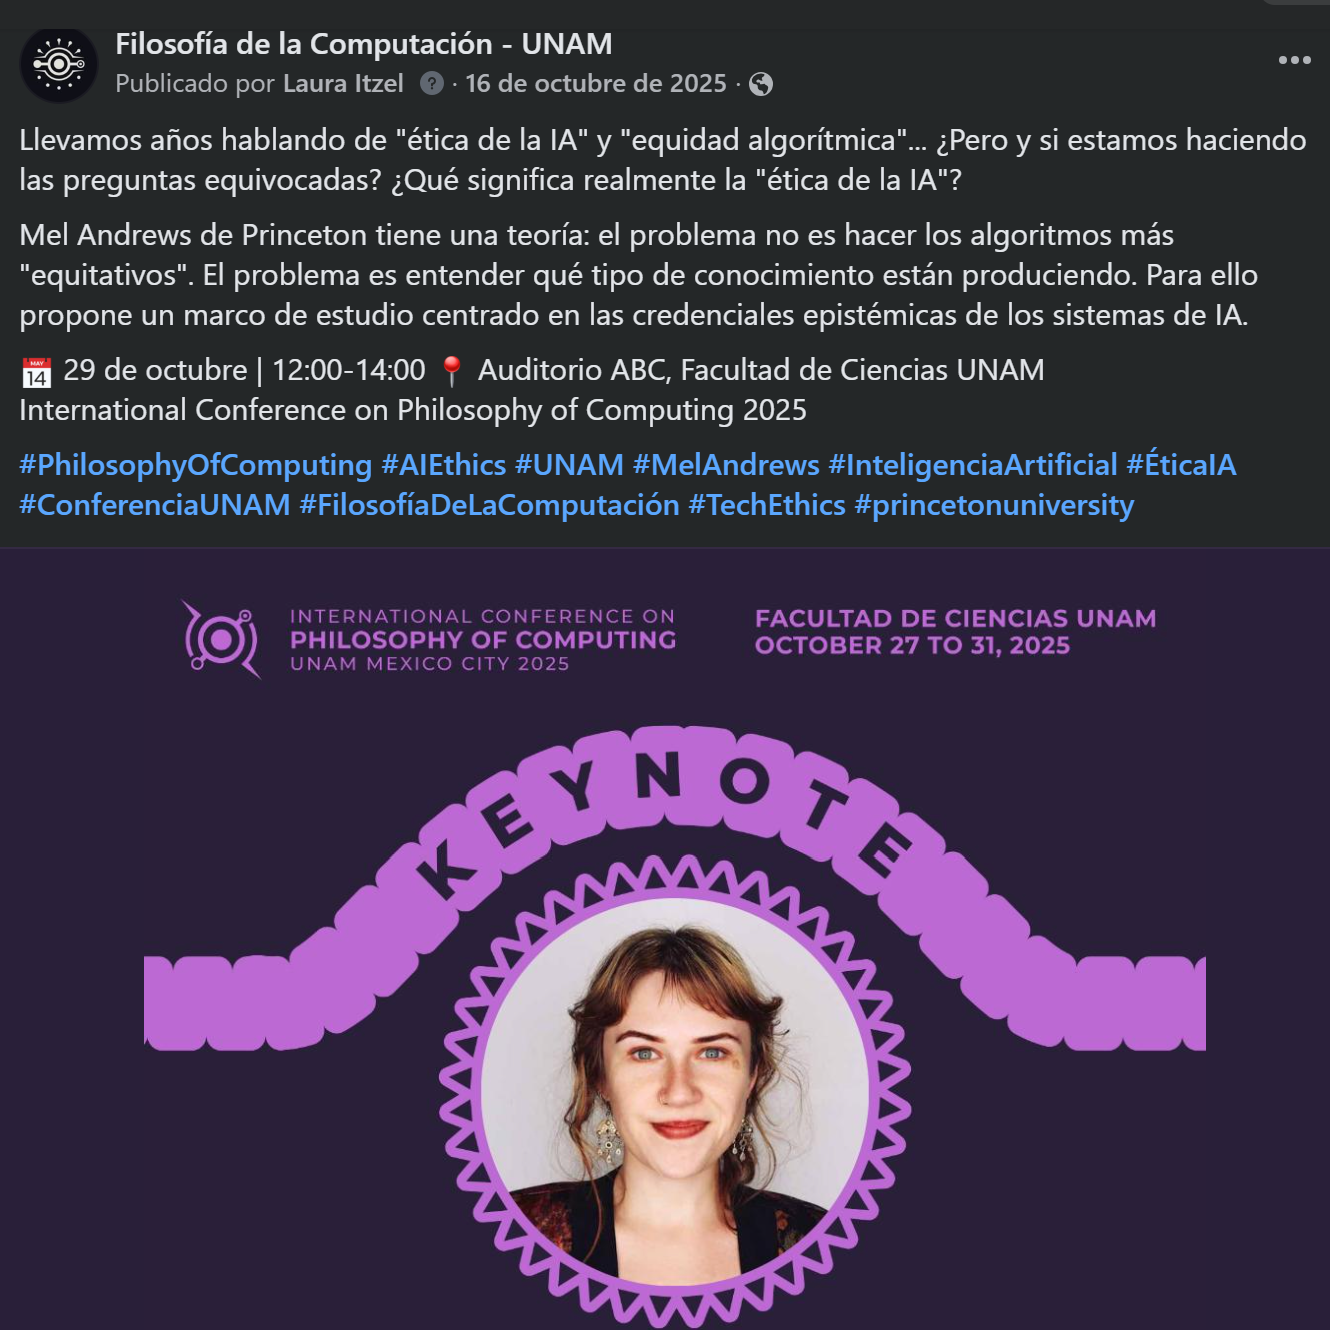
\includegraphics[width=\linewidth]{images/post3.png}
    \end{minipage}\hfill
    \begin{minipage}{0.24\textwidth}
        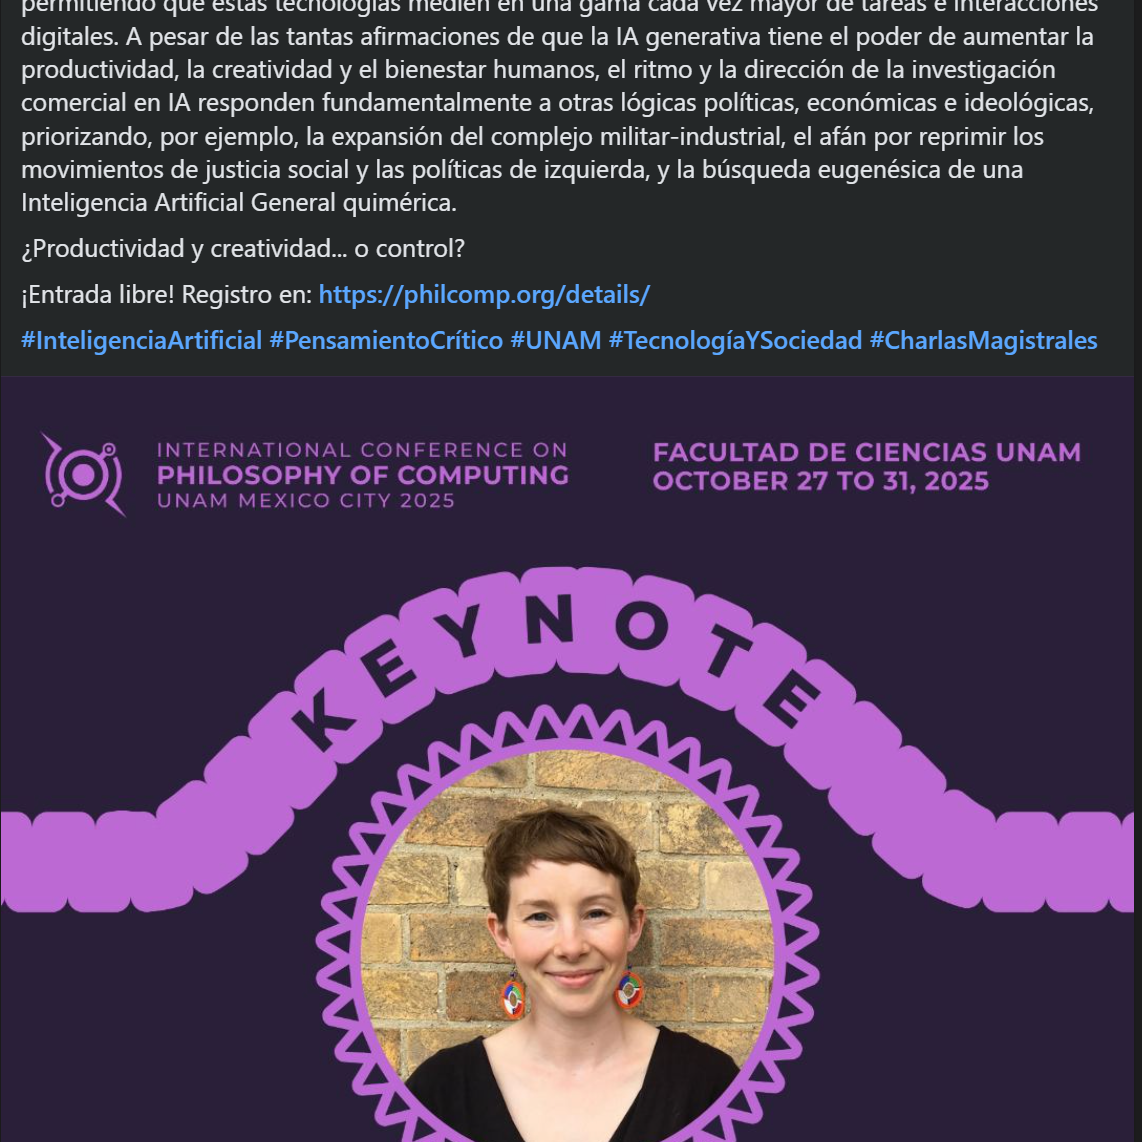
\includegraphics[width=\linewidth]{images/post4.png}
    \end{minipage}

    \vspace{0.5em}

    \begin{minipage}{0.24\textwidth}
        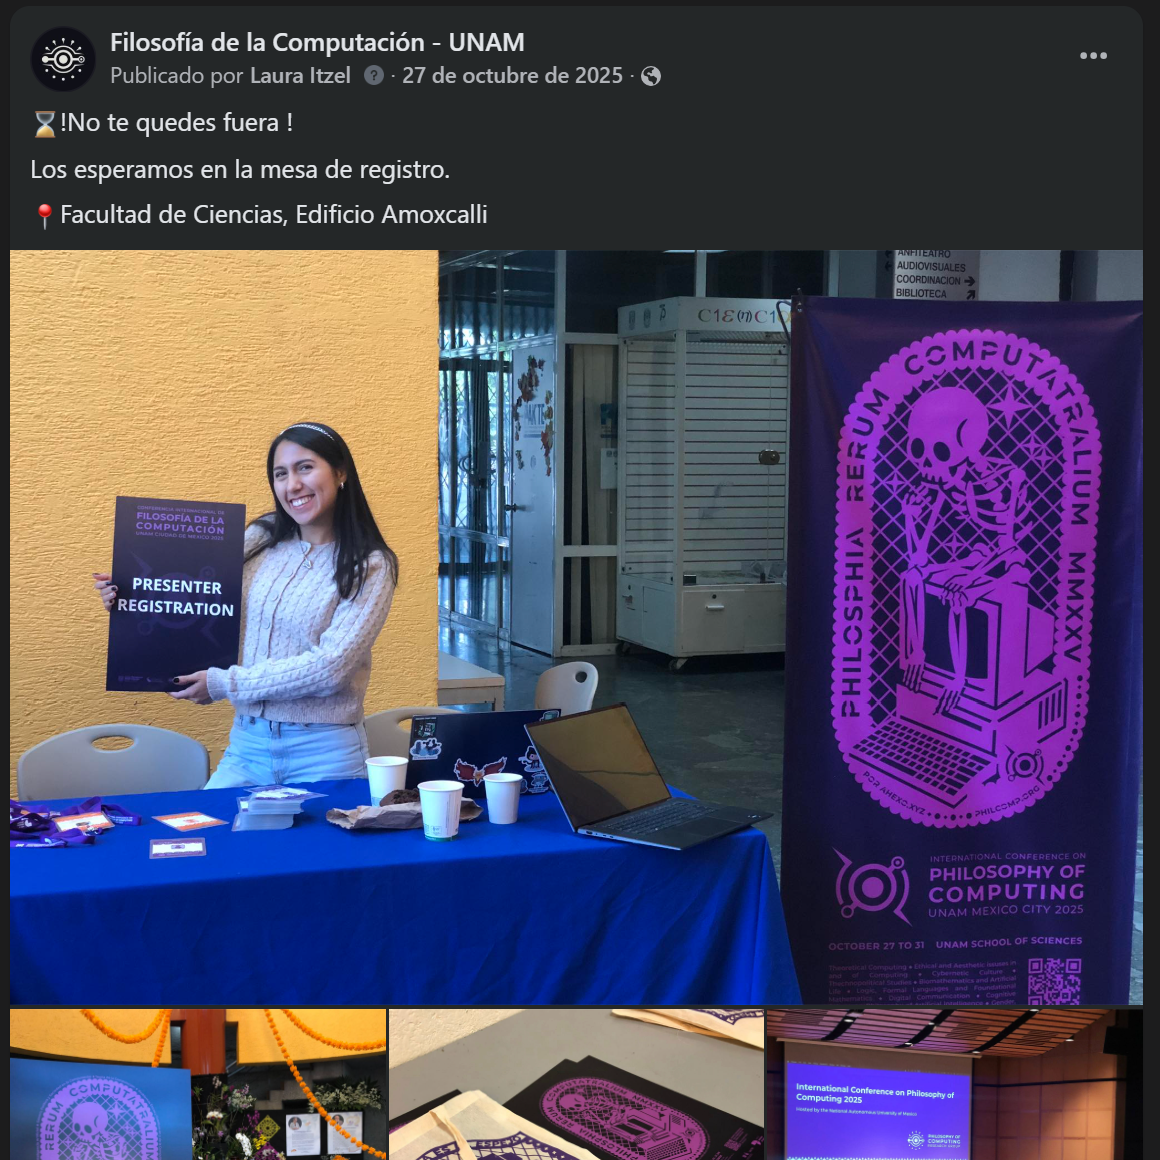
\includegraphics[width=\linewidth]{images/post5.png}
    \end{minipage}\hfill
    \begin{minipage}{0.24\textwidth}
        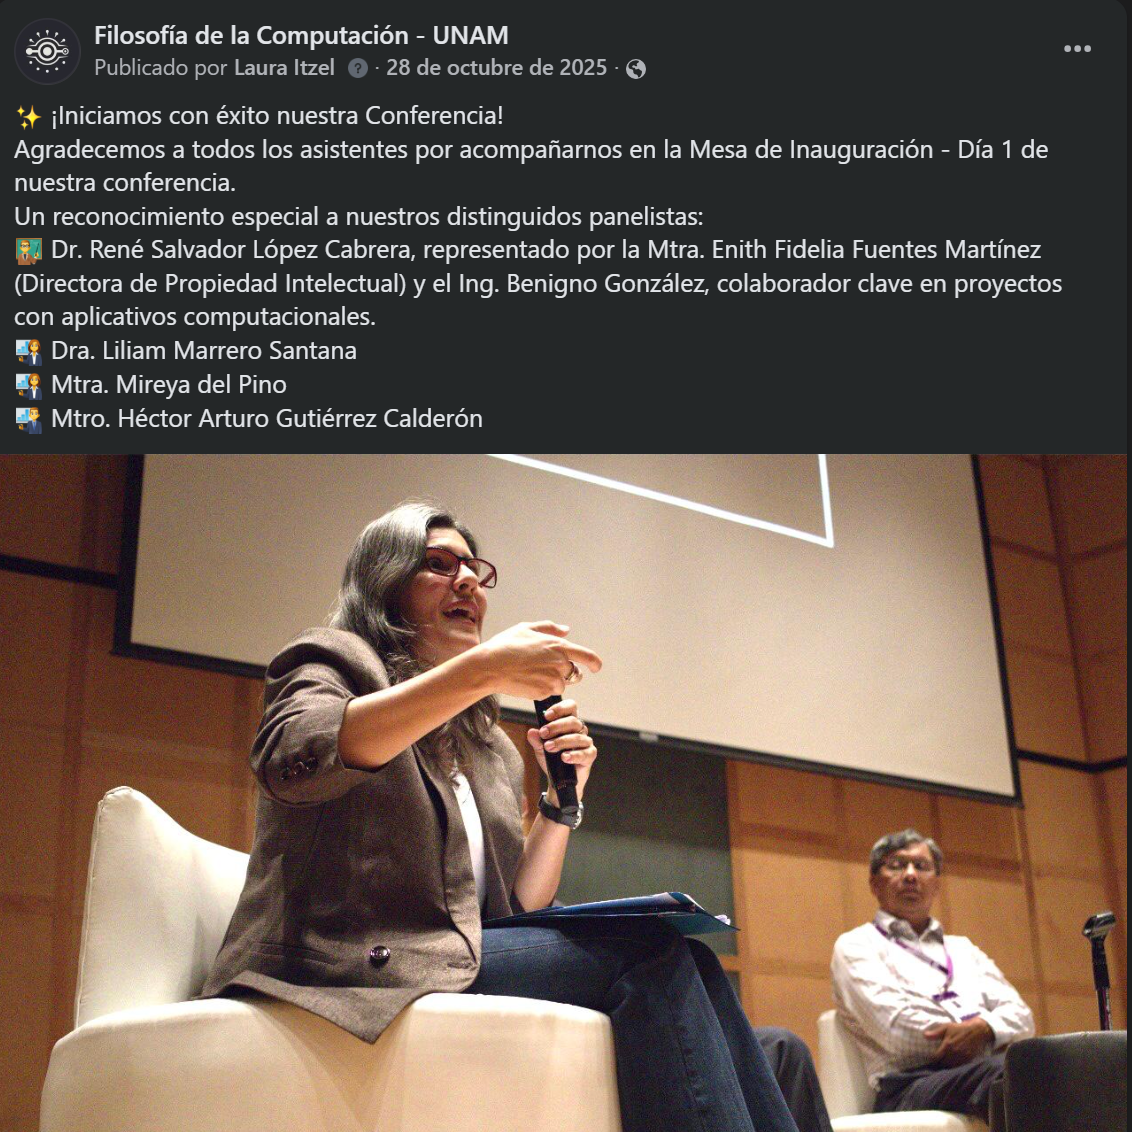
\includegraphics[width=\linewidth]{images/post6.png}
    \end{minipage}\hfill
    \begin{minipage}{0.24\textwidth}
        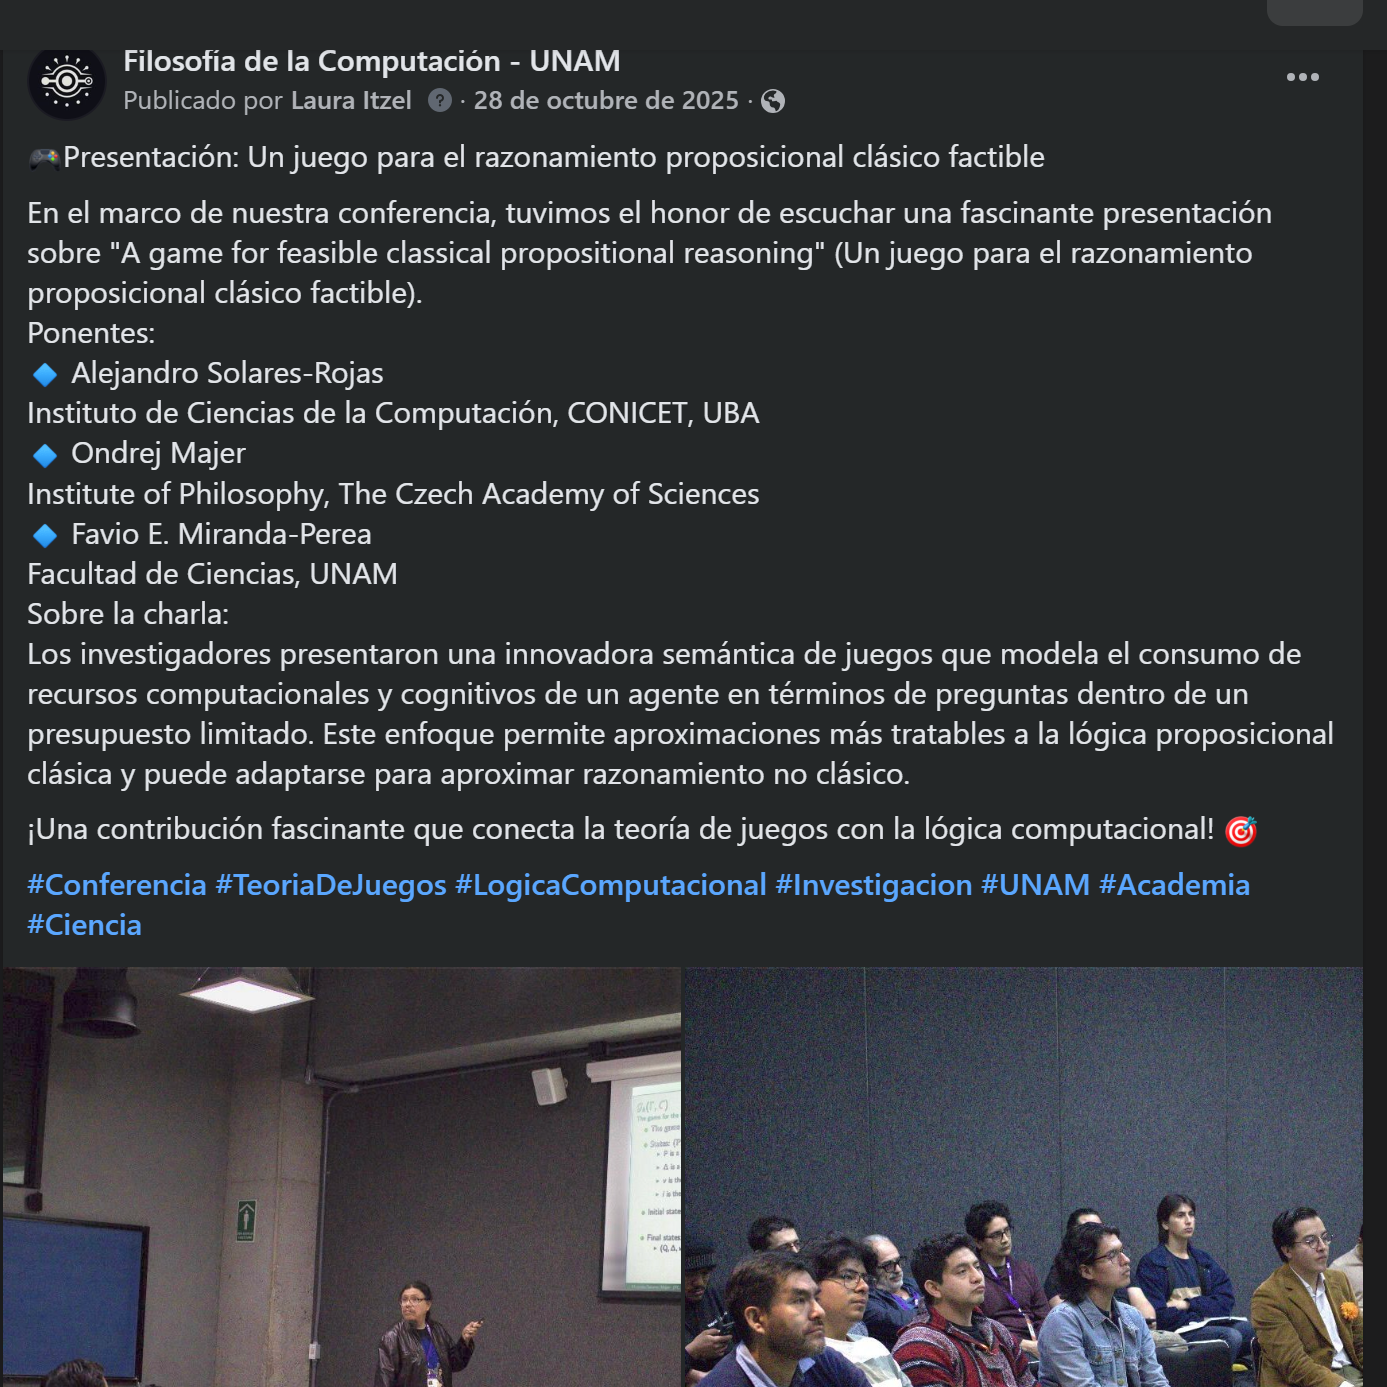
\includegraphics[width=\linewidth]{images/post7.png}
    \end{minipage}\hfill
    \begin{minipage}{0.24\textwidth}
        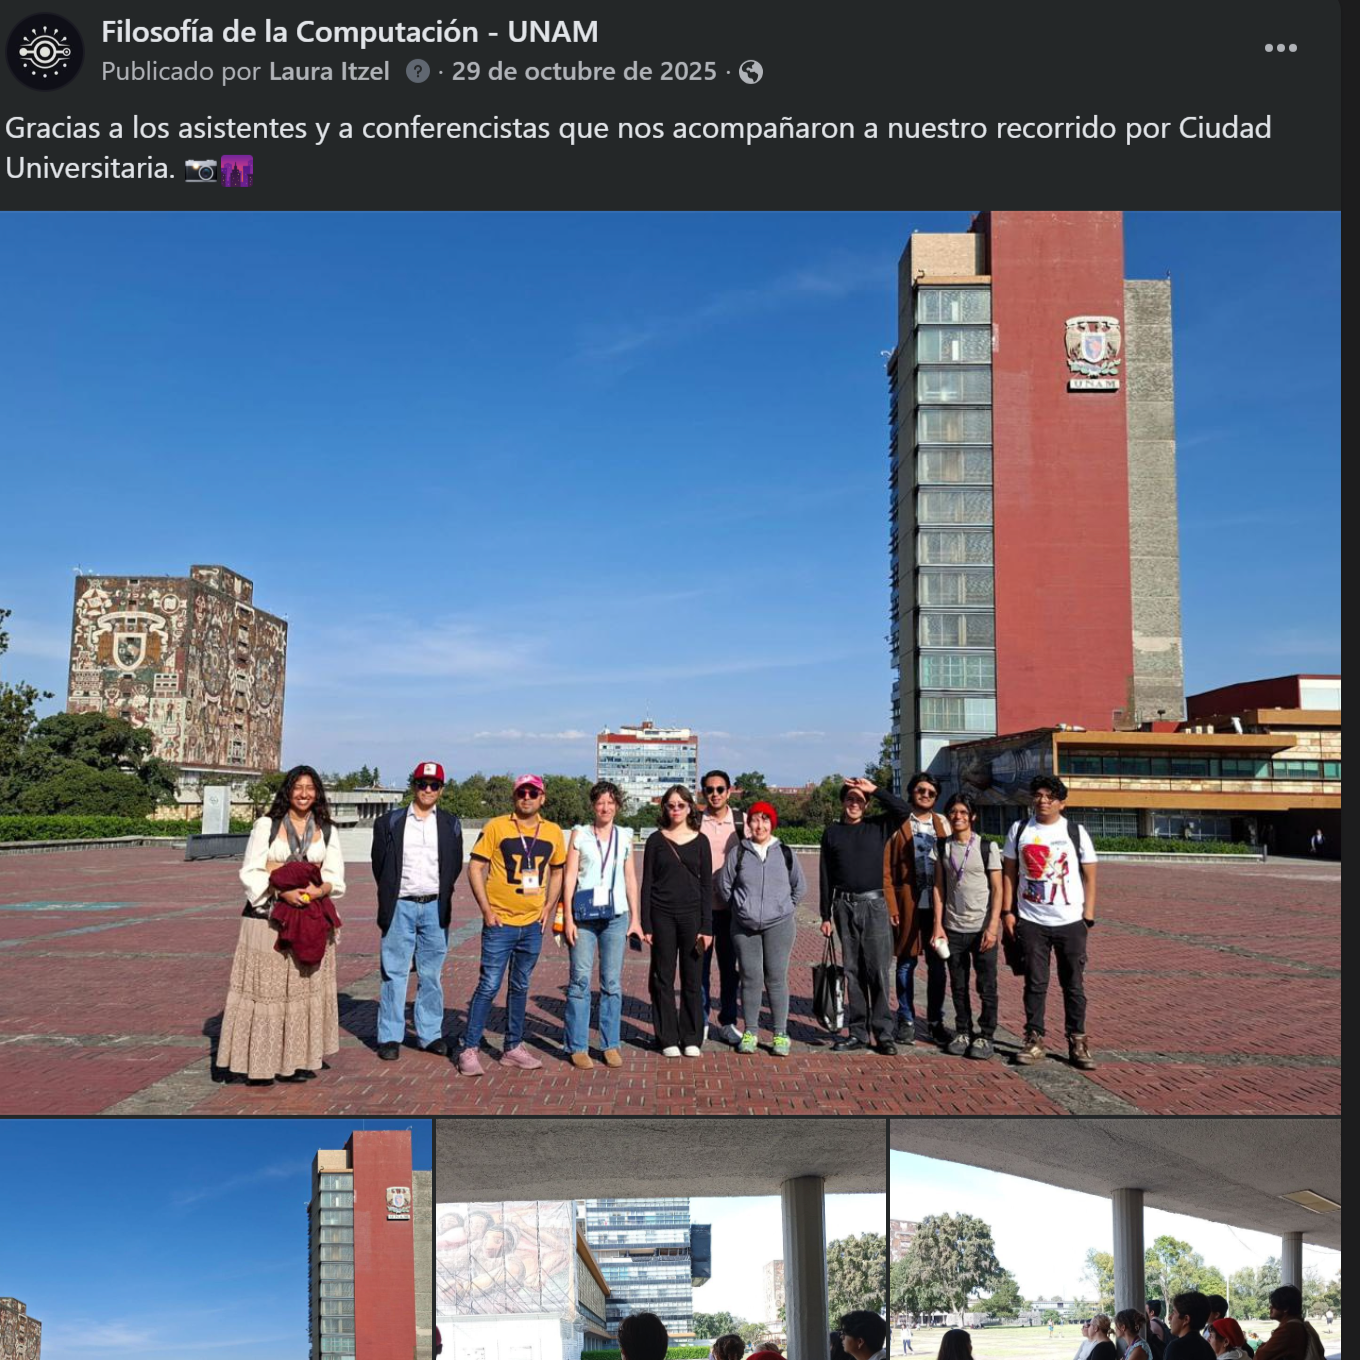
\includegraphics[width=\linewidth]{images/post8.png}
    \end{minipage}

    \vspace{0.5em}

    \begin{minipage}{0.32\textwidth}
        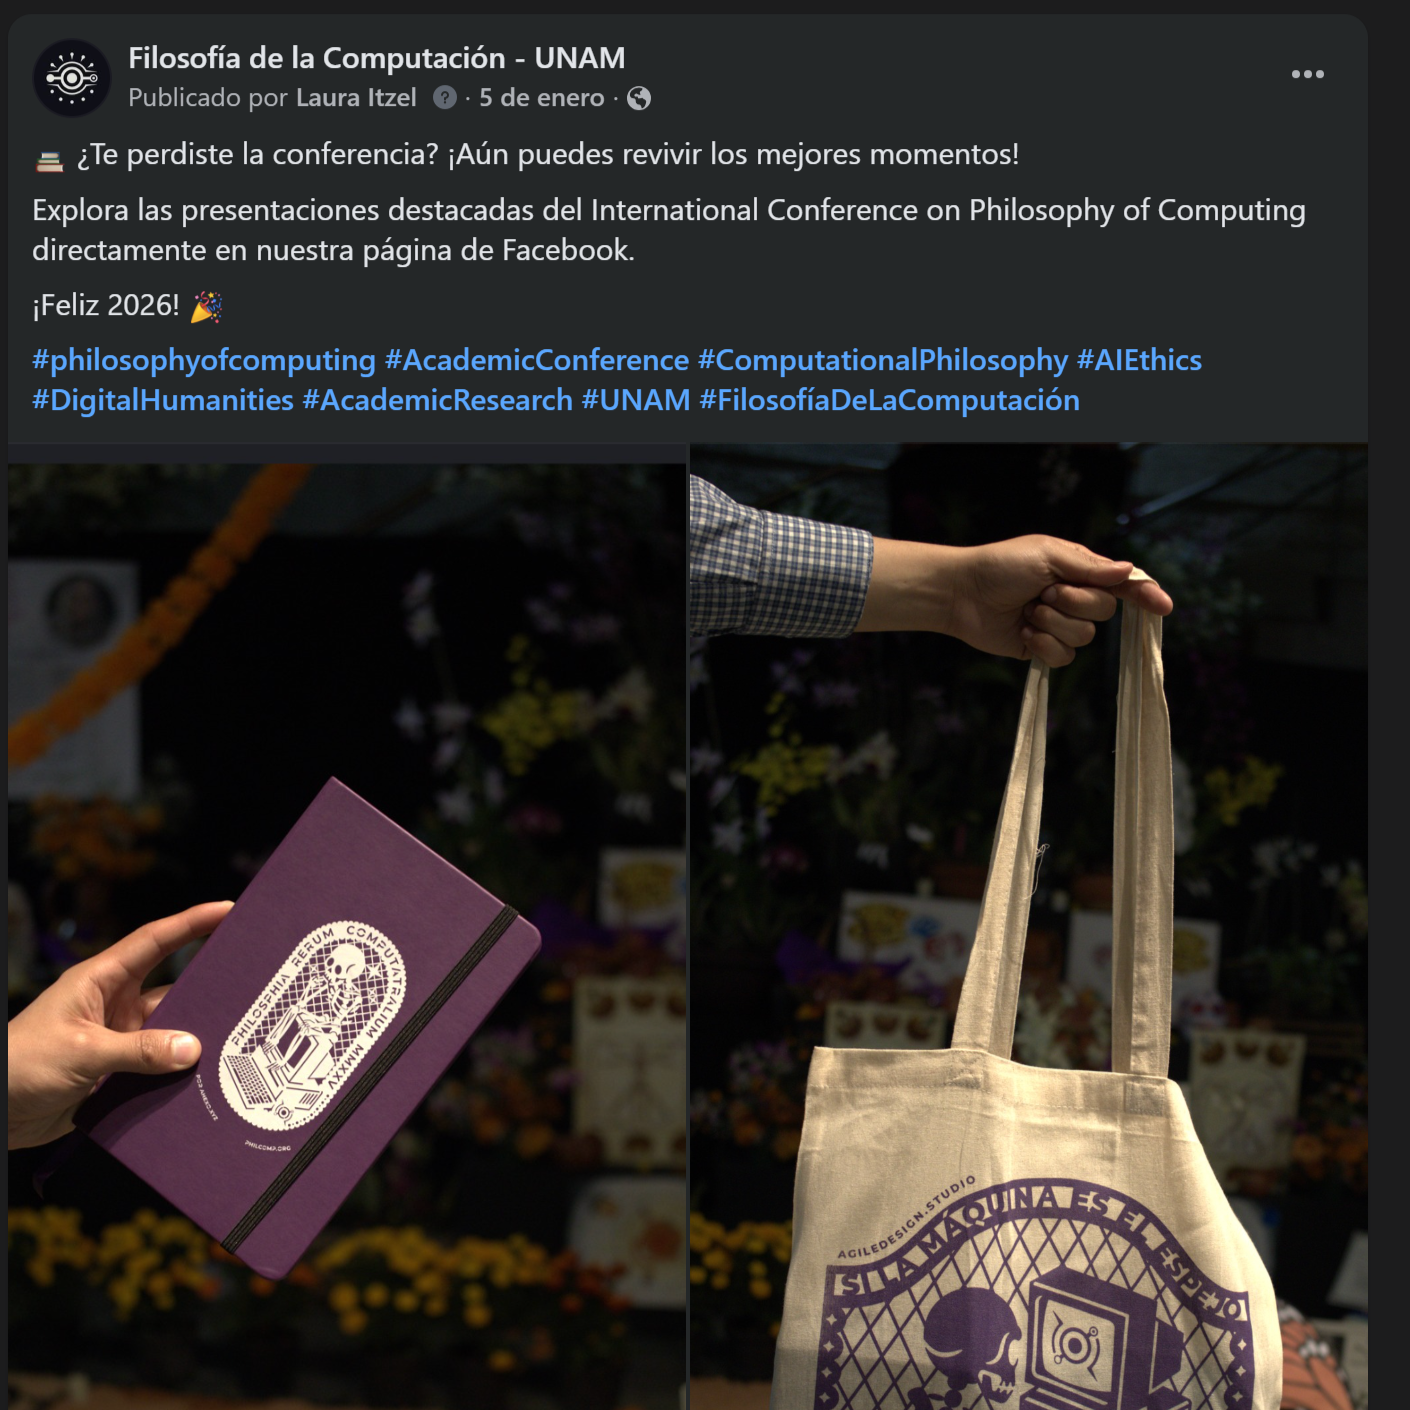
\includegraphics[width=\linewidth]{images/post9.png}
    \end{minipage}\hfill
    \begin{minipage}{0.32\textwidth}
        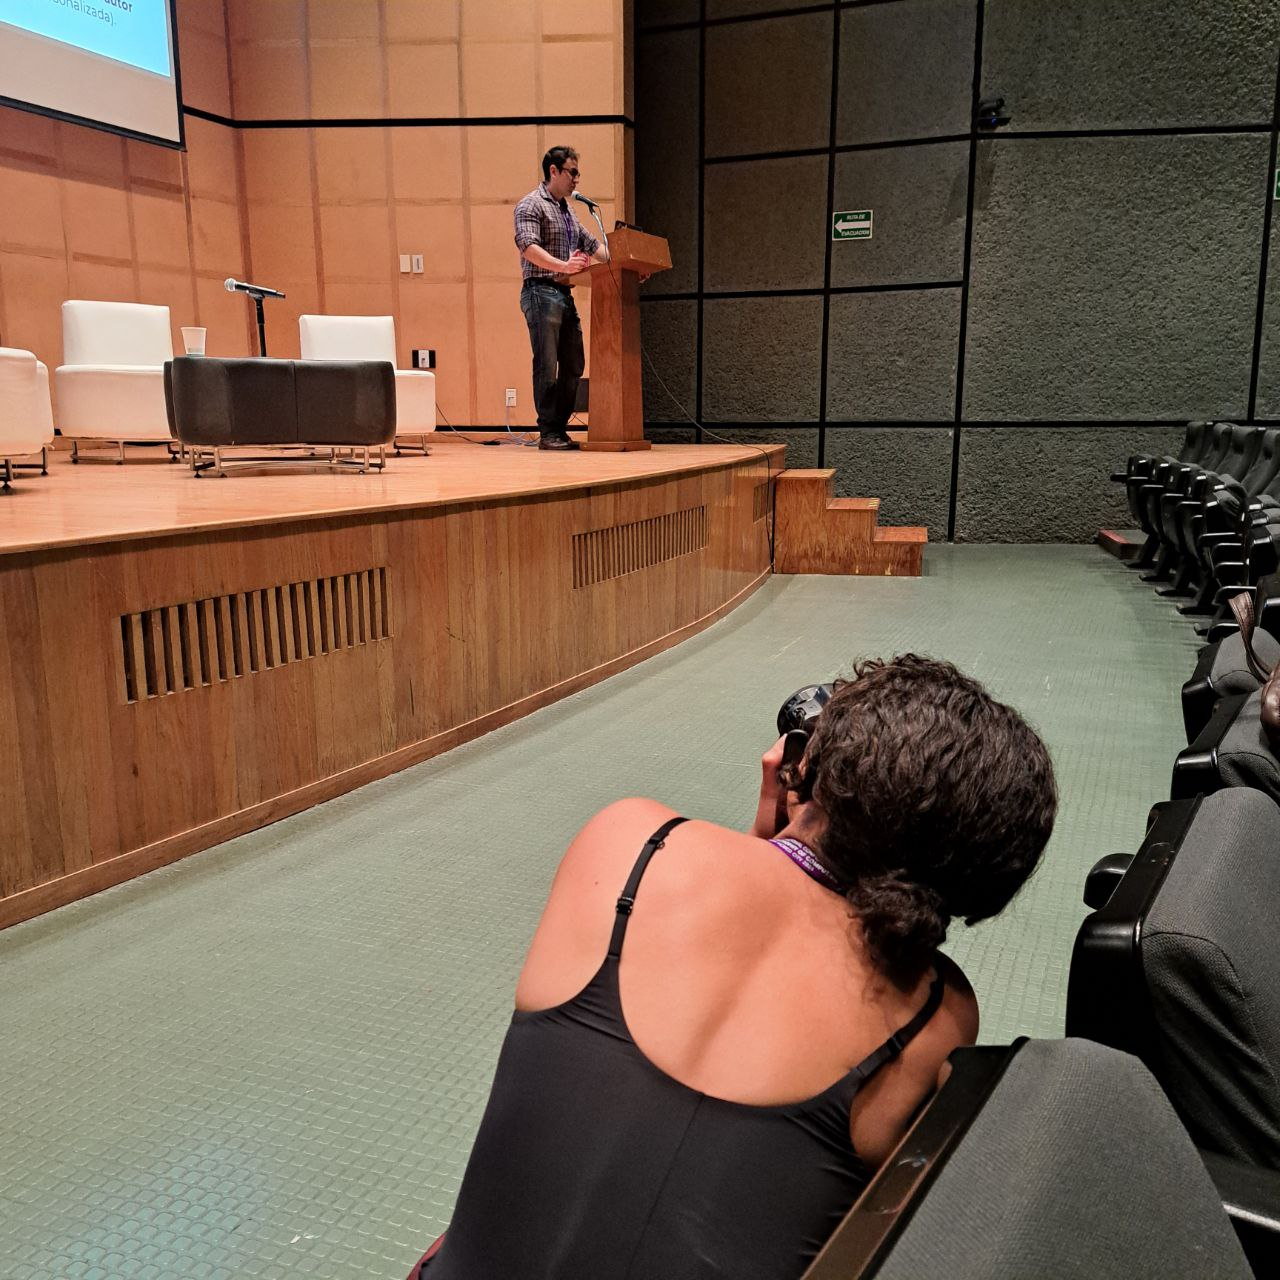
\includegraphics[width=\linewidth]{images/post10.jpg}
    \end{minipage}\hfill
    \begin{minipage}{0.32\textwidth}
        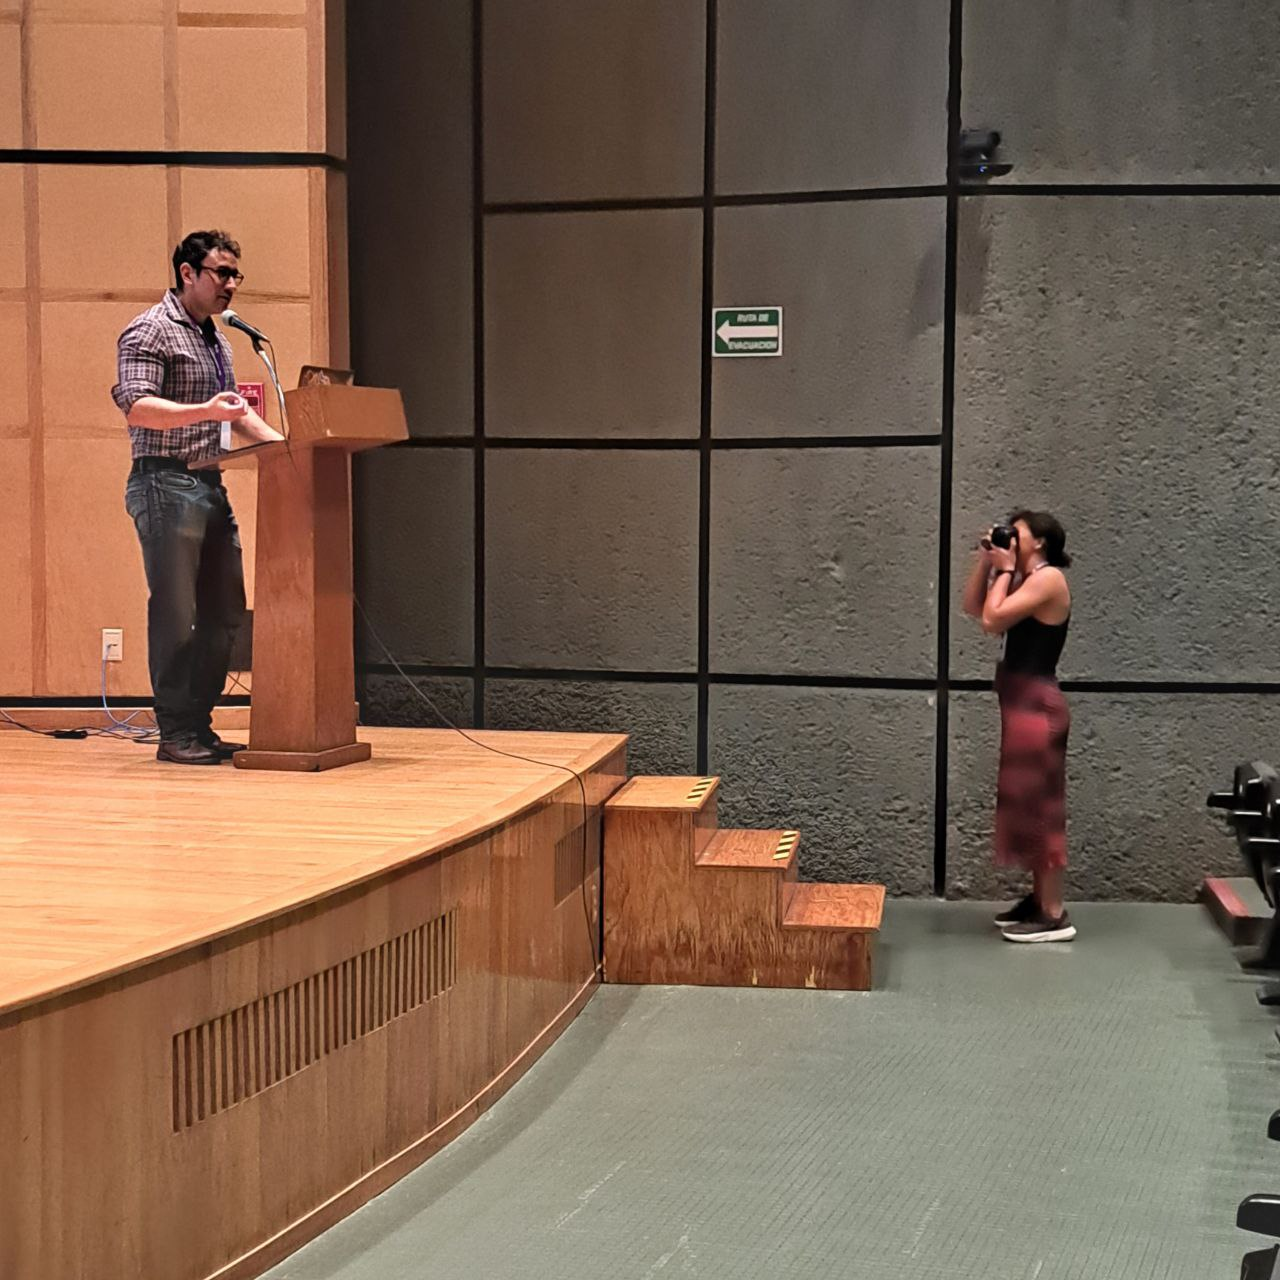
\includegraphics[width=\linewidth]{images/post11.jpg}
    \end{minipage}
\end{center}

\bigskip
\begin{center}
  Atentamente,\\
\end{center}
\begin{center}
    \begin{minipage}[t]{0.45\textwidth}
        \centering
        \rule{0.9\linewidth}{0.4pt}\\[0.5em]
        Laura Itzel Rodríguez Dimayuga \\
        Estudiante de Ciencias de la Computación
        Facultad de Ciencias, UNAM
    \end{minipage}\hfill
    \begin{minipage}[t]{0.45\textwidth}
        \centering
        \rule{0.9\linewidth}{0.4pt}\\[0.5em]
        M. en Fil. C. Enrique Francisco Soto Astorga \\
        Profesor de Asignatura “A”
        Facultad de Ciencias, UNAM
    \end{minipage}
\end{center}

\vspace{0.5cm}

\noindent Ciudad Universitaria a 6 de abril de 2026, Ciudad de México.

\end{document}
